\begin{figure}[h]
    \centering
    \begin{subfigure}{.5\textwidth}
      \centering
      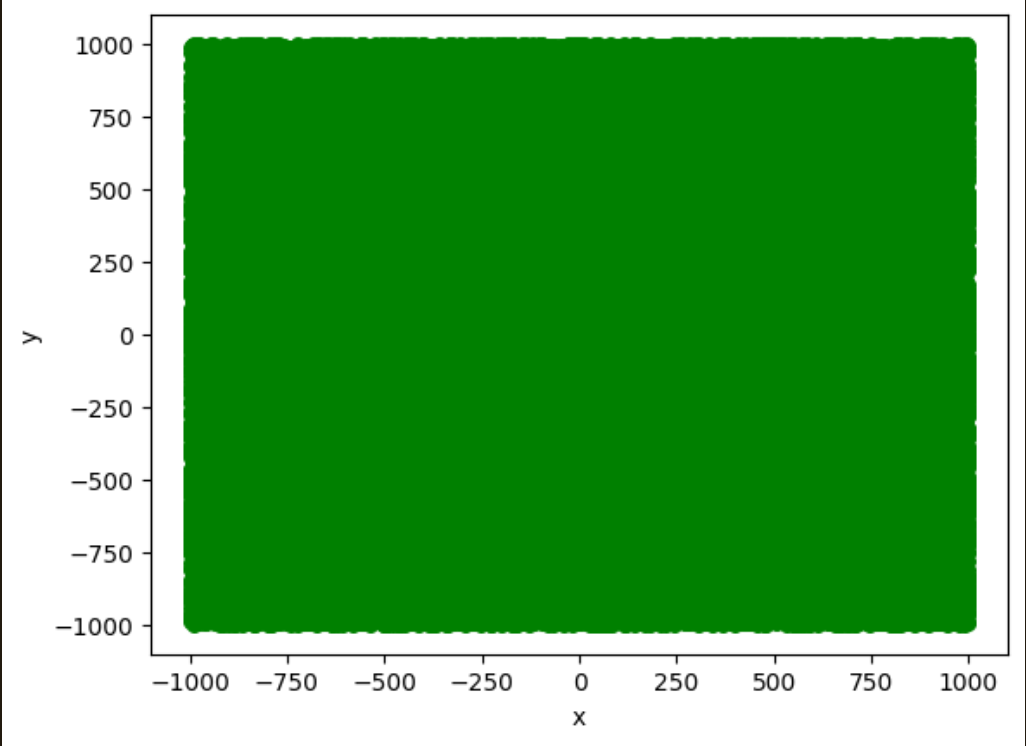
\includegraphics[width=.9\linewidth]{1.png}
      \caption{$10^5$ losowych punktów $(x, y) \in \left[-1000,1000\right]^{2}$.}
      \label{fig:sub1}
    \end{subfigure}%
    \begin{subfigure}{.5\textwidth}
      \centering
      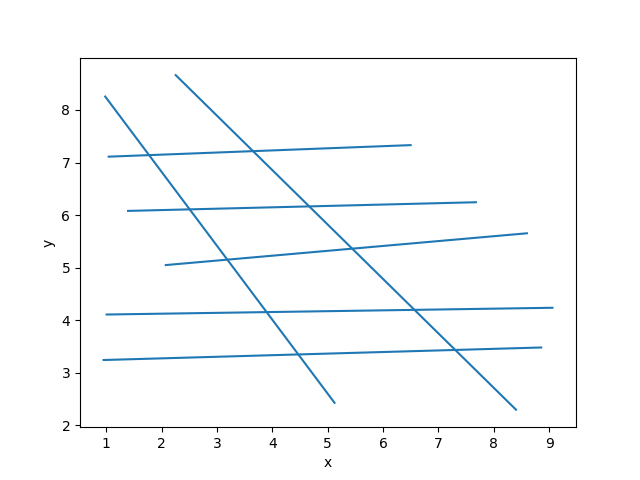
\includegraphics[width=.9\linewidth]{2.png}
      \caption{$10^5$ losowych punktów $(x, y) \in \left[-10^{14},10^{14}\right]^{2}$.}
      \label{fig:sub2}
    \end{subfigure}
    \label{fig:test}
    \end{figure}
    
    \begin{figure}[h]
    \centering
    \begin{minipage}{.5\textwidth}
      \centering
      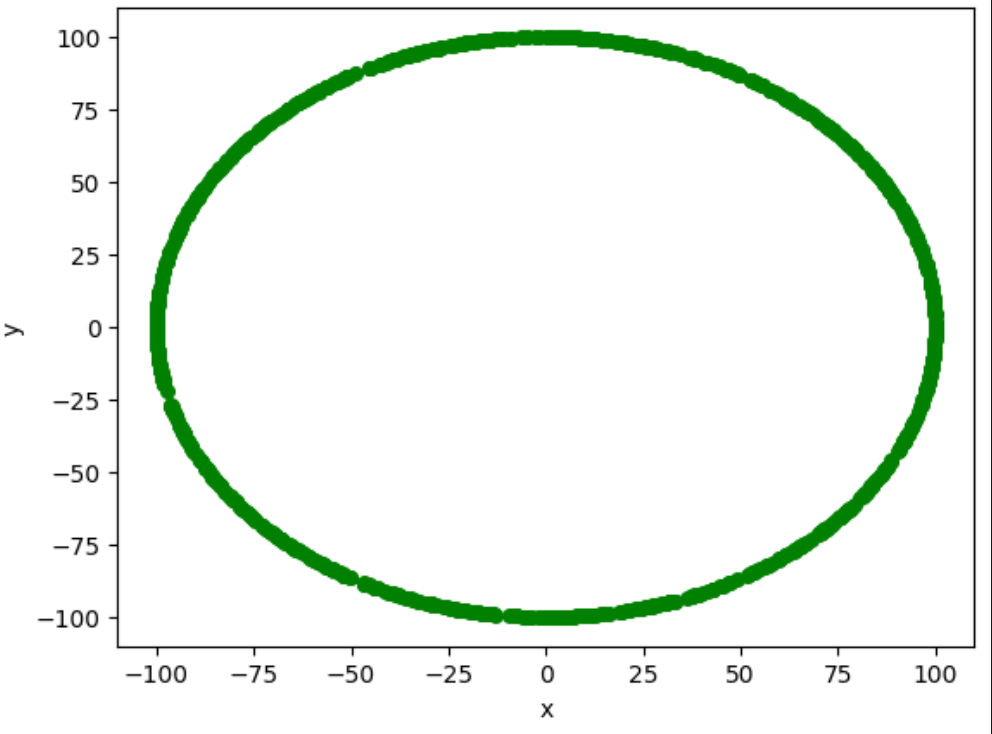
\includegraphics[width=.9\linewidth]{3.png}
      \caption{$1000$ losowych punktów leżących na okręgu.}
      \label{fig:test1}
    \end{minipage}%
    \begin{minipage}{.5\textwidth}
      \centering
      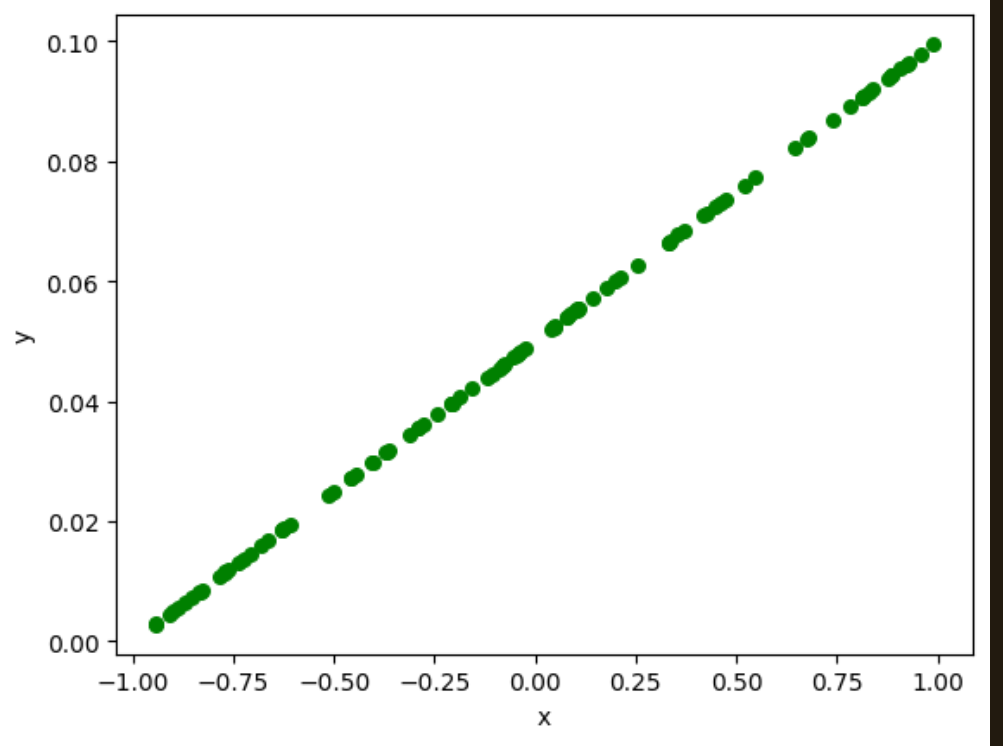
\includegraphics[width=.9\linewidth]{4.png}
      \captionof{figure}{$ 1000$ losowych punktów na prostej.}
      \label{fig:test2}
    \end{minipage}
    \end{figure}

    \subsection{Algorytmy generacji zbiorów}
\quad 1. Dla zbiorów a i b.
 \begin{lstlisting}
  def generate_uniform_points(left, right, n = 10 ** 5):
    points = []
    for i in range(n):
        x = np.random.uniform(left, right)
        y = np.random.uniform(left, right)
        points.append((x, y))

    return points
\end{lstlisting}
\par
2. Dla zbioru c.
\begin{lstlisting}
  def generate_circle_points(O, R, n = 1000):
    points = []
    for _ in range(n):
        angle = 2 * np.pi * np.random.uniform()
        points.append((R * np.cos(angle), R * np.sin(angle)))
    return points
\end{lstlisting}
\par
3. Dla zbioru d.
\begin{lstlisting}
  def generate_collinear_points(a, b, n=100):
    points = []
    xt = b[0] - a[0]
    yt = b[1] - a[1]
    for i in range(n):
        t = np.random.uniform()
        points.append((xt * t + a[0], yt * t + a[1] ))
    
    return points
\end{lstlisting}
\newpage